    \documentclass[usenames,dvipsnames]{report}

    \usepackage {a4}
    \usepackage [utf8] {inputenc}
    \usepackage [french] {babel}
    \usepackage {verbatim}
    \usepackage{amsmath,amsfonts,amssymb}
    %\usepackage {algorithm}
    \usepackage[french,lined,boxed,commentsnumbered]{algorithm2e}
    %\usepackage[french,boxed]{algorithm2e}
    %\usepackage {pst-node}
    %\usepackage{lmodern}
    %\usepackage[dvips]{color}
    \usepackage[usenames,dvipsnames]{color}
    \usepackage{gastex}
    \usepackage{fancyhdr}
    \usepackage{pstricks}
    \usepackage{multicol}
    \usepackage{graphicx}
    \usepackage{float}
    \usepackage{lastpage}

    %%%%%%%%%%%%%%%% Variables %%%%%%%%%%%%%%%%
    \def\titre{Etude comportementale
    du robot Vitirover}
    \def\filiere{Robotique}
    \def\annee{$3^{ème}$}  % $1^{ere}$, $2^{eme}$ ou $3^{eme}$
    \def\anneescolaire{2012/2013}
    \def\promotion{2013}
    \def\equipe{Chapron Jeremy\\Boudinet Florian\\Morillon Antoine}
    \def\encadrant{Denis Lapoire, Gregoire Passault} 
    %%%%%%%%%%%%%%%%%%%%%%%%%%%%%%%%%%%%%%%%%%%


    \pagestyle{fancy}
    \rfoot{\textit{Année \anneescolaire}}
    \cfoot{\thepage/\pageref{LastPage}}
    \renewcommand{\headrulewidth}{0.4pt}
    \renewcommand{\footrulewidth}{0.4pt}

    \newcommand{\HRule}{\rule{\linewidth}{0.5mm}}

    \begin{document}

    \begin{titlepage}

    \begin{center}


    % Upper part of the page
    %
\includegraphics[width=0.3\textwidth]{logo.eps}\\[1cm]

    \textsc{\LARGE ENSEIRB-MATMECA}\\[1cm]

    \textsc{\Large {Filière \filiere, \annee année}}\\[0.5cm]
    \textsc{\Large {Promotion \promotion}}\\[0.5cm]

    % Title
    \HRule \\[0.4cm]
    { \huge \bfseries \titre}\\[0.4cm]
    Simulateur de terrain et de déplacements pour le robot Vitirover
    \\
    \HRule \\[1.5cm]

    % Author and supervisor
    \begin{minipage}{0.4\textwidth}
    \begin{flushleft} \large
    \emph{Auteurs :}\\
    \equipe
    \end{flushleft}
    \end{minipage}
    \begin{minipage}{0.4\textwidth}
    \begin{flushright} \large
    \emph{Encadrant :} \\
    \encadrant
    \end{flushright}
    \end{minipage}

    \vfill

    % Bottom of the page
    {\large \today}

    \end{center}

    \end{titlepage}



    \tableofcontents
    %\thispagestyle{fancy}

    \chapter{Introduction}
    Dans le cadre de la production du robot Vitirover et dans le but de pouvoir effectuer des tests sur les déplacements du robot, notamment sur son algorithme de déplacement, il nous a été demandé d’implémenter un simulateur pour le robot. 

    Au travers de ce rapport, nous expliquerons les démarches effectuées ainsi que les solutions techniques apportées lors de la création de ce simulateur.
    L’objectif premier de ce simulateur est de générer un terrain qui respecte les critères majeurs d’une parcelle de vigne. Pour cela il faut bien entendu modéliser les imperfections du terrain ainsi que les pieds de vignes et piquets les maintenant droits sans oublier le robot lui même. Une fois le terrain généré et répondant bien aux critères d’une parcelle, nous nous intéresserons aux différentes stratégies de déplacement envisageable pour le robot.
    Tout au long du développement du simulateur, nous nous sommes assurés que le code développé soit bien modulaire et que donc qu’il serait facile de venir y greffer un nouvel algorithme de déplacement ou bien de nouveaux paramètres concernant la forme ou bien la nature du terrain.


    Dans un premier temps on parlera de la création du terrain. Puis, dans une seconde partie nous verrons comment le robot est implémenté et paramétré puis nous décrirons les algorithmes de déplacement que nous avons mis en place. Et enfin, nous parlerons de la façon dont les paramètres sont fournis et programmes et des fichiers de configuration. Pour finir nous envisagerons les améliorations possibles à ce simulateur pour le rendre encore plus fonctionnel.
    %\thispagestyle{fancy}

    \chapter{Interface Graphique et rendu OpenGL}

    Notre simulateur utilise OpenGL pour faire le rendu 3D, et le framework Qt pour l’interface graphique, le contrôle des éléments et le rendu de la fenêtre.
    Qt fournit une classe de base, QGLWidget, afin de faciliter l’intégration d’OpenGL dans une fenêtre Qt.


    Nous avons pris garde lors de la conception de bien séparer le code de la simulation, de sa représentation graphique et de l’interface. Ainsi, nous disposons d’un ensemble de classes qui permettent soit de représenter une objet de la simulation, soit d’effectuer son rendu 3D.
    Par exemple, la Simulation est modélisée par la classe Simulation, et sont rendu 3D par la classe SimulationViewer. Il est important de bien séparer le graphique du code métier, afin de faciliter la conception et la maintenance. De plus, si un jour le besoin d’utiliser un autre moteur qu’OpenGL et Qt se présente, la transition en sera facilitée.


    \section{Architecture}
    Notre simulateur se compose d’une fenêtre principale, représentée par la classe MainWindow, qui elle même se décompose en plusieurs composantes. L'élément central contient le Widget de représentation OpenGL. Un dock est disposé sur la droite de la fenêtre afin de contenir les différents éléments de contrôles. Ces éléments permettent d’afficher différentes informations utiles a l'utilisateur, comme par exemple la position du robot. Mais aussi pouvoir jouer sur les paramètres, comme la génération de la carte, l'affichage des pieds de vigne ou non, ou encore faire varier la vitesse de la simulation.


     Un timer est intégré au programme principal pour permettre l’appel aux fonctions de rafraîchissement des éléments graphiques, mais surtout pour effectuer un “tour” de simulation supplémentaire. 

    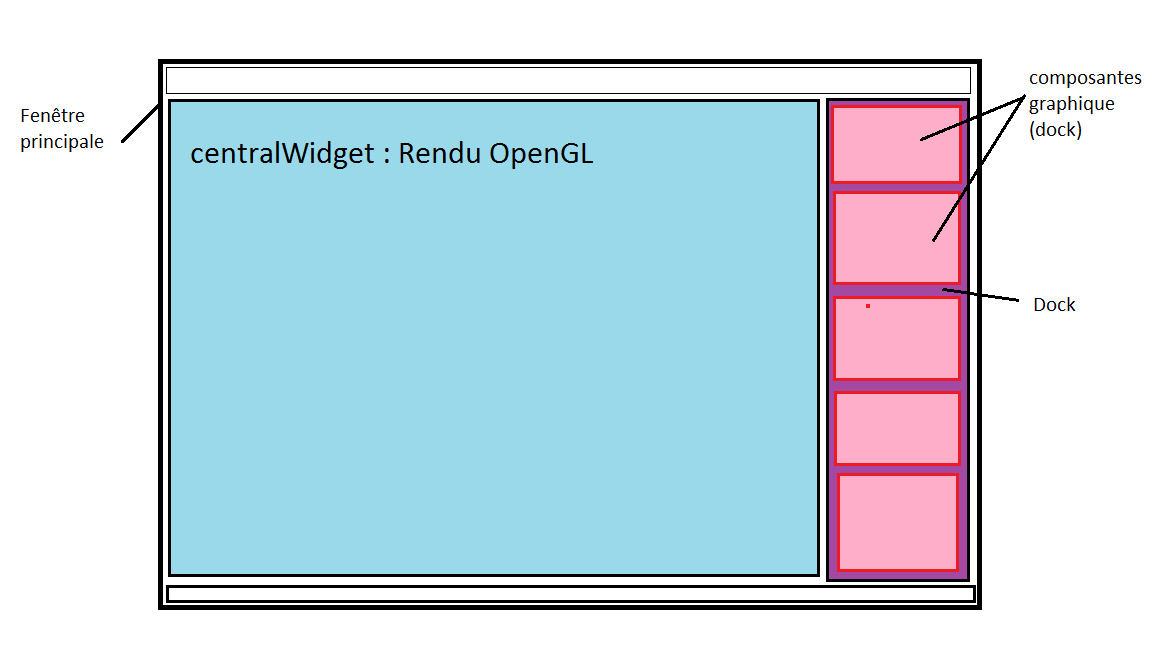
\includegraphics[width=12cm]{GUI-vitirover.png}


    \textit{Architecture de l interface} 

    \section{Représentation des éléments}
    Notre simulation nécessite la représentation d’un certain nombre d'éléments essentiels à la bonne visualisation de la simulation et sa compréhension.


    Il est nécessaire de discrétiser la parcelle de vigne, et de définir une cote de conversion entre taille réel de l'élément et sa représentation graphique.  Ainsi, le terrain généré est représenté par un ensemble de carrés de 5cm de largeur. Une unité de simulation se convertie donc en 5cm réels. Cette échelle a le mérite d'être assez petite pour pouvoir représenter un jeune cep, un obstacle tel qu’un cailloux ou autre branchage. Cette unité ne doit pas être trop petite, sinon la complexité temps/espace deviendrait bien trop grande, pour un gain de représentation minime (peu ou pas d'élément plus petit que 5cm à représenter).

    \chapter{Génération de terrain}
    Un des points important pour la simulation est l’utilisation d’un terrain représentatif d’une parcelle de vigne. 
    Il est important que ce terrain soit diffèrent à chaque fois, et soit produit de manière “aléatoire”.

     L’idée de base consistant à générer des hauteurs aléatoires sur toute une carte, est bien entendu mauvaise, et le résultat produit désastreux, sans le moindre réalisme. 
     Il est possible de représenter notre terrain a l’aide d’une heightmap, où le niveau de gris représente la hauteur.


\bigskip
\\
    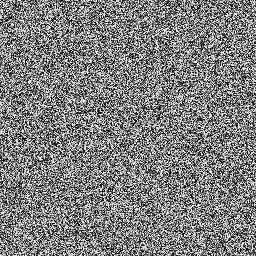
\includegraphics[width=7cm]{alea.png}


    \textit{HeightMap aleatoire} 

\bigskip
    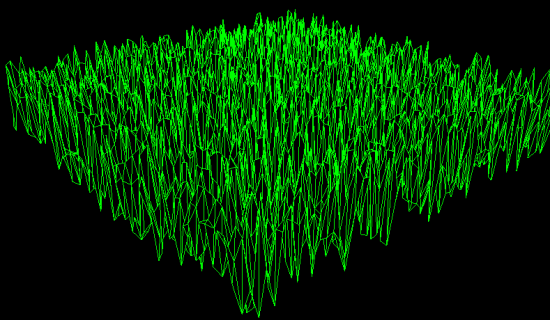
\includegraphics[width=10cm]{screen_alea-miniature.png}


    \textit{HeightMap aleatoire 3D} 

    Il a donc fallu trouver un algorithme pouvant générer un terrain “réaliste”, en particulier pour une parcelle de vigne.
    Après avoir effectué des recherches, on a  noté qu’il n’en existe pas beaucoup. 
    Le domaine d'activité ayant le plus besoin de ce type d’algorithme est le secteur du jeu vidéo. Le but étant de générer des cartes aléatoires et le plus réaliste possible. L’exemple type est sans nul doute Minecraft ou SimCity.
\\

    Le choix s’est alors porté sur le bruit de Perlin, sûrement celui le plus utilisé et le plus simple à mettre en oeuvre.
    

    L'idée de l'algorithme de Perlin est d'affiner un terrain par itérations successives tout en interpolant entre les valeurs connues.
    La génération commence en fixant quelques valeurs aléatoires à intervalle régulier puis en interpolant tous les autres points à partir de ces valeurs.
\\

     A ce stade là, le résultat commence à ressembler à un terrain, mais il n'est pas très naturel. Il va falloir ensuite lui ajouter des "calques" successifs pour affiner la pente 
     du terrain et lui donner un aspect réaliste.
    On peut assimiler ce mécanisme à la notion d’harmoniques. A chaque calque, le nombre de valeurs de hauteur sélectionnées est passé au carré, 
    mais leur coefficient (poids) est réduit. Ainsi, on se retrouve avec une multitude de valeurs réparties sur la carte, chaque valeur ayant un coefficient
     d’importance en fonction du “calque” auquel elle appartient. Il suffit ensuite de fusionner les différents calques en faisait des interpolations, sans oublier,
      bien évidement, de tenir compte du poids des valeurs.

\\

\bigskip

    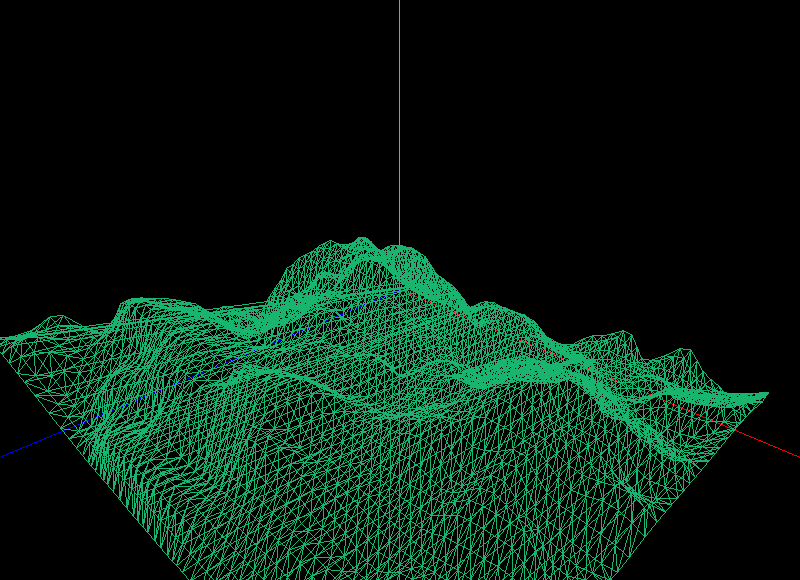
\includegraphics[width=10cm]{gene-map4.png}


    \textit{Représentation 3D } 
\\

\bigskip

\\


    On  peut jouer sur trois paramètres de l’algorithme, afin d’obtenir différents types de carte.
    \begin{itemize}
        \item Le nombre de calques utilisés : plus le nombre de calques sera grand, plus la carte comprendra du bruit.
        \item La fréquence : le nombre de valeurs sélectionnées sur la carte.
        \item La persistance (poids) : plus la persistance initiale sera grande, plus l’image sera bruitée, car les calques inférieurs auront un poids non négligeable.
    \end{itemize}

\\


    Le dernier point important est la définition de l'intervalle de valeur pour la hauteur. Notre parcelle ne peut pas avoir un dénivelé trop grand, il est donc important que l'écart entre la hauteur minimale et maximale ne soit pas trop grand.


\\
    Il nous reste ensuite à représenter les pied de vigne et les piquets afin d’avoir une parcelle réaliste.

     
    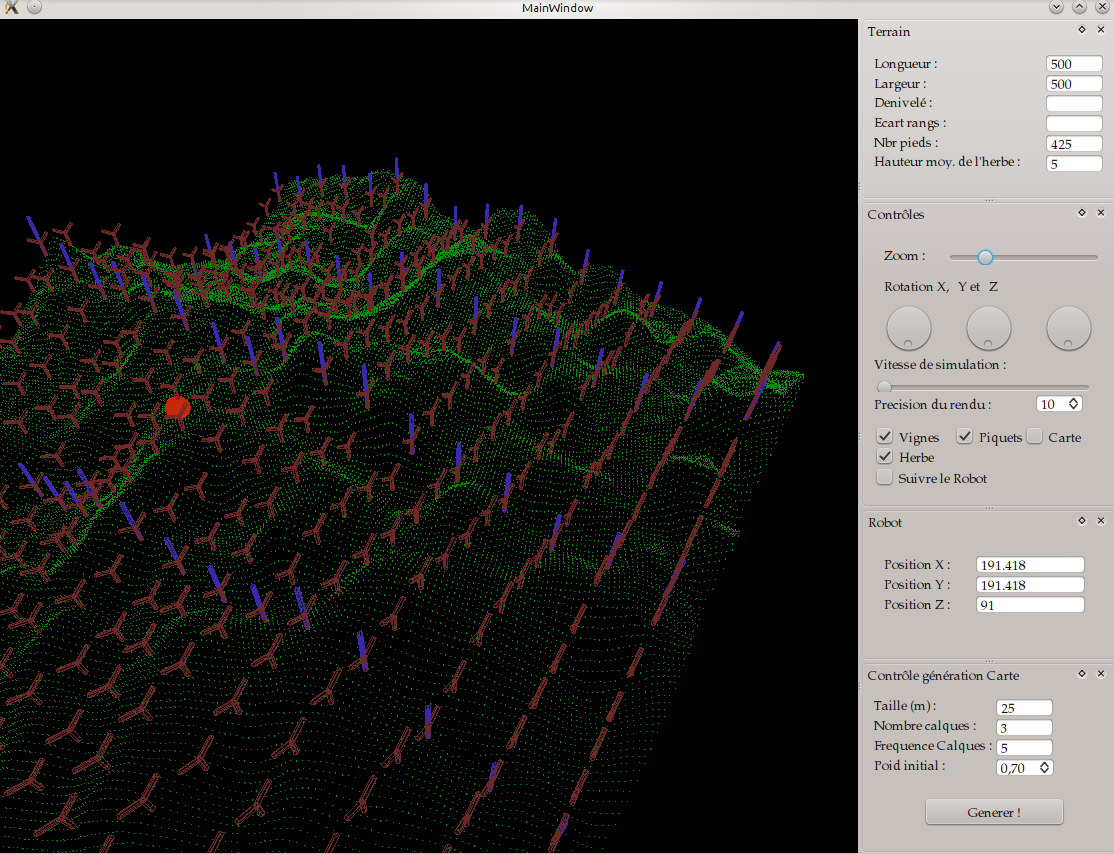
\includegraphics[width=12cm]{final.png}


    \textit{Représentation Finale} 

     
    \chapter{Paramètrage du robot}
    Chaque robot dispose d’un ensemble de paramètres pour le définir tels que ses dimensions (length, width, height, weight), 
    la position de son centre de gravité sur la carte (center) sous le type Point que nous avons implémenté afin de gérer des coordonnées sur trois axes; 
    la vitesse de l’engin ainsi que son accélération sous la forme d’un vecteur (en utilisant la classe Point : speed, acceleration ). 
    Le prochain objectif spatial est aussi retenu (xobjectif, yobjectif). Un robot ayant des limitations matérielles dans ses déplacements (puissance des moteurs), 
    ses vitesses et accélérations sont limitées, ainsi on retient dans la classe les valeurs des normes maximales de ces vecteurs (maxSpeed, maxAcceleration ).
\\


     Bien que la viscosité n’ait pas encore été exploitée, un paramètre permet d’estimer une valeur à partir de laquelle il ne pourra plus se déplacer, 
     par exemple pour un embourbement total nécessitant une intervention extérieure pour le récupérer (coeff), un autre à partir duquel il se déplacera 
     mais avec difficulté (déplacement à moitié efficace (coeffMoitie). 
\\     
     
     Enfin dans une optique de diversités stratégiques, un paramètre retient le type
      d’action en cours, par exemple aller au centre de la carte, ou retourner au point de départ, qui pourra être amélioré en “tonte active”, “
      rechargement de batteries nécessaire”, “déplacement jusqu’à une zone de coupe sans tonte pendant le parcours”.
       
\\

    Cependant certains de ces paramètres n’ont qu’un sens relatif tant qu’ils ne sont pas utilisés avec des valeurs réelles.
     Dans une utilisation future, une estimation empirique serait la bienvenue. D’autres valeurs ne sont pas implémentées en
      tant que paramètres afin de ne pas complexifier encore plus, en particulier le nombre de tranches de temps nécessaires à atteindre l’asymptote de la vitesse.

    \chapter{Algorithme de déplacement}


    L’algorithme de déplacement est l’objectif majeur de la finalité de ce projet. 
    Le simulateur a été implémenté avec comme objectif secondaire d’être réutilisable par l’équipe de R&D de Vitirover.
    La simulation se charge de déplacer les différents robots à un intervalle de temps fixe.
     Pour se faire, elle demande à chaque robot de réfléchir à un objectif de positionnement,
      par exemple d’avancer simplement d’une case en x et en y, ou encore d’aller au milieu de la carte. Puis le robot est chargé de se tourner dans la bonne direction, et enfin la simulation calcule en fonction des vitesse et accélération, position, voire viscosité du terrain le déplacement du robot.
\\

    Les choix de déplacement du robot et ses déplacements effectifs sont indépendants. Le robot choisit là où il veut aller après un calcul sur les informations bruitées qu’il obtient en analysant son environnement avec ses capteurs. Ensuite le simulateur se charge de déplacer le robot en conséquence, il détecte les moments auxquels le robot collisionne et l’informe de l’impossibilité du déplacement. De plus, le simulateur introduit des biais en déplaçant le robot approximativement par rapport à ses objectifs théoriques. Ceci est dû au fait que la modélisation physique de l’environnement n’est que partielle donc son résultat pratique n’est pas nécessairement le même et empiriquement on constate que les déplacements ne sont effectivement pas optimaux. Cette partie du projet reste à développer.
\\

        Sur la simulation actuelle, on peut voir le vitirover se déplacer en ligne droite vers le centre de la carte jusqu’à une distance de quelques unités et faire demi-tour vers sa position originelle, encore une fois jusqu’à une certaine distance et ce en boucle. Bien que les collisions soient repérées elles ne sont pas encore évitées.
        
    \chapter{Fichiers de configuration}
    Dans le but de stocker les données utiles au programme et de pouvoir modifier ces données 
    sans avoir à recompiler le projet, nous avons décidé de stocker des informations via des 
    fichiers de configuration. Le format pour lequel nous avons opté est le format YAML (YAML Ain’t Markup Language). 
    \\
    
    L’idée derrière le langage YAML est que toute donnée peut-être représentée sous la forme de listes, tables de hachages
     et données scalaires. Dans notre cas nous utiliserons les listes d’associations pour stocker nos données.
        Un fichier de configuration différent est disponible pour chaque partie du projet. 
        
        Voici ci dessous un exemple de fichier YAML concernant le robot:
    \begin{verbatim}
    {
    name: Vitirover,
    length: 1000,
    width: 500,
    height: 500,
    weight: 1500,
    maxSpeed: 1.0,
    maxAcceleration: 0.2
    }
    \end{verbatim}


    L’avantage d’utiliser une structure de données comme celle ci est le fait que l’on peut accéder aux valeurs utiles en faisant une recherche par nom. La structure est comparable a celle d’un dictionnaire. Pour traiter ces données nous utilisons la bibliothèque yaml-cpp qui est une bibliothèque C++ contenant les fonctions utiles relatives au traitement des fichiers YAML. En se basant sur cette bibliothèque, nous avons mis en place une fonction read qui permet, en connaissant le nom de l’attribut que l’on veut lire, de récupérer sa valeur.

        
    \chapter{Optimisations possibles}
    Le simulateur est fonctionnel et permet de voir un premier déplacement du robot, 
    mais bien évidemment on peut envisager bon nombre d’améliorations possibles. 
    Le premier point sur lequel on pourrait ajouter du contenu est le robot lui même.
     En effet on pourrait lui ajouter des capteurs de différentes natures et effectuer 
     des mesures au cours du déplacement. ceci permettrait de tester les relevés effectués 
     par les capteurs du robot sans avoir à l’envoyer en situation pseudo-réelle.
     
     
        D’autre part, on peut envisager une plus grande richesse des paramètres 
        utilisés pour décrire le terrain. En effet on pourrait y ajouter des informations
         concernant la nature du terrain (herbe, terre, caillou …)  ou bien encore 
         conserver en mémoire les points auxquels le robot a rencontré des difficultés
          dans son déplacement.
          
          \\
          
        Pour finir on peut améliorer l’algorithme de déplacement du robot dans le but de
         tester différents algorithme et de récolter des statistique quant à la surface de tonte couverte. Cette dernière optimisation peut-être envisagée dans le cadre d’un nouveau projet de recherche d’algorithme optimal pour le robot.

    \chapter{Conclusion}
    Tout au long de ce rapport, nous avons présenté les solutions techniques que nous avons utilisé dans le développement de ce simulateur. Au final il permet de visualiser un terrain cohérent ainsi que le robot se déplaçant sur celui-ci mais il reste encore des améliorations qui peuvent lui être apportées. En revanche, nous avons fait notre possible pour que ce projet serve de base solide au développement d’un simulateur complet et tout le travail effectué a donc respecté un soucis de modularité et de clarté du code. Il en va de même pour l’algorithme de déplacement qui contient les mouvements de base comme avancer et tourner  et il est donc facile de venir lui greffer un algorithme plus complexe en partant de ses mouvements de base.
        Au final, nous nous sommes attaqués à la plupart des aspects de ce projet relativement riche en possibilités malgré les difficultés que nous avons rencontré. Le simulateur en l’état actuel est fonctionnel et peut-être repris pour être enrichi. 
        
    \chapter{Bibliographie}

    \begin{itemize}
        \item http://www.codecolony.de/opengl.htm#Introduction
        \item http://newbiz.developpez.com/tutoriels/opengl/heightmap/
        \item http://en.wikipedia.org/wiki/Perlin\_noise
        \item http://minecraft.fr/generation-du-terrain-partie-1/
        \item http://vterrain.org/Elevation/Artificial/
        \item http://paulboxley.com/blog/2011/03/terrain-generation-mark-one
    \end{itemize}

    \end{document}


